\documentclass[]{spieman}

\usepackage[utf8]{inputenc} \usepackage{amsmath,amsfonts,amssymb}
\usepackage{graphicx} \usepackage{grffile} \usepackage[colorlinks=true,
allcolors=blue]{hyperref} \usepackage{pdflscape} \usepackage{afterpage}

% Title definition
\title {The WIYN One Degree Imager in 2018: An Extended 30-Detector Focal Plane
and Operational Challenges}

\author[a,b]{Daniel R. Harbeck} \author[c]{Mike Lesser} \author[b]{Wilson Liu}
\author[d]{Bob Stupak} \author[d]{Ron George} \author[d]{Ron Harris}
\author[d]{Gary Poczulp} \author[d]{Jayadev Rajagopal} \author[e]{Ralf Kotulla}
\author[c]{David Ouellete} \author[e]{Eric Hooper} \author[e]{Michael Smith}
\author[e]{Dustin Mason} \author[f]{Peter Onaka} \author[f]{Greg Chin}
\author[d]{Emily Hunting} \author[d]{Robert Christensen}

\affil[a]{Las Cumbres Observatory, Goleta, CA (USA)} \affil[b]{WIYN Observatory,
Tucson, AZ (USA)} \affil[c]{The University of Arizona, Tucson, AZ (USA)}
\affil[d]{NOAO, Tucson, AZ (USA)} \affil[e]{University of Wisconsin, Madison, WI
(USA)} \affil[f]{University of Hawaii, Honolulu, HI (USA)}

\newcommand{\electron}{e$^-$\xspace} \newcommand{\degree}{$^\circ$\xspace}


\begin{document}

\maketitle

\begin{abstract}
    
We report on the performance of the upgraded One Degree Imager (ODI) at the WIYN
3.5 meter telescope at the Kitt Peak Observatory. The focal plane has been
expanded by additional sixteen detectors in spring / summer 2015. The now thirty
Orthogonal Transfer Array CCD detectors has a field of view of 40’ x 48’ on the
sky. The newly added detectors underwent a design revision to mitigate reduced
charge transfer efficiency under low light conditions (fat zero problem). We
discuss the imaging performance and challenges in the photometric calibration of
the wide field of view, helped by the addition of telescope baffles. In a
parallel project, we upgraded the instrument's filter mechanism, where a
degrading worm-gear mechanism was replaced by a chain drive that is operating
faster and at a higher reliability level. Two more filters, a U band and narrow
band filter were added to the instrument's complement. We will review the
lessons learned during nearly three years of operating the instrument in the
observatory environment and discuss infrastructure upgrades that were driven by
ODI's needs. 

\end{abstract}


%>>>> Include a list of keywords after the abstract

\keywords{Ground based instrumentation, wide field imaging, CCD, Orthogonal
    Transfer Array, Observatory Operations}

%%%%%%%%%%%%%%%%%%%%%%%%%%%%%%%%%%%%%%%%%%%%%%%%%%%%%%%%%%%%%
\section{Introduction}
The One Degree Imager (ODI) has been the major instrument development project from 2004 to 2016 for 
the WIYN 3.5 meter telescope (Kitt Peak, Arizona), and its design has been documented in various
SPIE articles\cite{jacoby2002,Harbeck2008,Jacoby2008,Yeatts2008,Harbeck2010,Yeatts2010,harbeck2014,gopu2014,}. 
The instrument is designed for a one degree  square field of view with 64 Orthogonal Transfer
Array (OTA) CCD sensor. A first incarnation of ODI 
was deployed in the summer of 2012 with a partially populated focal plane (with 13 out of 64 
detectors installed); this  incarnation of ODI was called pODI and was described in detail the SPIE 
Astronomical Telescopes + Instrumentation conference in 2014\cite{harbeck2014}. 

In that paper we outlined an incremental upgrade path for the instrument to a larger focal plane, 
and in 2015 we have deployed ODI with am enlarged 5x6 detector array by adding 17 new detectors; 
this incarnation of ODI is generally referred to "5x6 ODI" or simply ODI, as now additional 
development of the focal plane is anticipated at this time.


\section{Upgrade of the Focal Plane}

\subsection{Detector performance}

* low light level CTE fixed (already confirmed in 2014 paper)

* amplifier glow unchanged

* residual charge remains and is fixed in the pipeline software code.  

\cite{Lesser2012}

* note on temperature stability, and possible limit on the number of viable detectors has been 
reached.

* crosstalk as before, only intra-detector, but not between detectors operated on same controller; 
new information since pODI only had one CCD attached per controller. 



\subsection{Tuning the acquisition software}

The ODI data acquisition is described in detail in previous SPIE contributions\cite{Yeatts2008,Yeatts2010}.
In short, the focal plane is read out by 20 Stargrasp CCD controllers which
interface to a network switch via 20 separate 1GB ethernet over fiber
connections. The switch itself bundles the data connection into a 10GB network
backbone used by the ODI computers (three 24 core, 32GB RAM servers). The stream
from the 30 CCDS is collected by a single server / java virtual machine that is
managed by a JBOSS 5 application server. The data are stored to disk.

The amount of data has more than doubled (from 13 detectors to now 30), and as
the detectors are read out in parallel, so has the data rate. The scalability of
the data acquisition system was tested before the upgrade by creating a mock-up
focal plane  configuration to simulate the enlarged focal plane. This test
revealed some bottlenecks: the interval between sustained bias readouts
increased from about 25 seconds to over 40 seconds. Several bottlenecks in the
data acquisition code were identified and mitigated during the upgrade project
and commissioning phase:


\begin{enumerate} 
    
\item Initially, all data were stored to a NFS mounted Oracle storage appliance
(ZFS....), and the data time to write fits files to disk was the major factor to
slow down the data handling process. As a mitigation we equipped the acquisition
server with a Raid 5 configured local storage array, utilizing only disks with a
6G interface. The imaging data were then slowly transfered by a background
process to the storage appliance, both as a mid-term storage and to stage data
for transfer into the ODI data archive.

\item  The simultaneous receiving of the data streams from 30 detectors posed no
major challenge over the 10GB network backbone.  However, when writing the the
data to disk we realized a significant  improvement in the write speed by
limiting the number of data streams that are written in parallel to disk. As a
mitigation, the FITS file writing routine was changed into a Callable that would
be submitted to a multi-threaded Executor with 10 threads. An additional
improvement in write performance was achieved by rewriting the fits io package
to allow writing into BufferedOutputfile,

\item As part of the data storage process, a thumbnail image is generated for
each detector to help the observer to judge image quality in real time. For
pODI, the thumbnail generation was delegated to a command line utility that was
called after the images were written to disk, reading back (and decoding) the
fits file again. Also, the thumbnail generation process was unnecessarily
serialized in the data acquisition process, i.e., telescope observations would
be blocked until thumbnail images were generated.  For 5x6 ODI we have moved the
thumbnail generation into the JVM, were the data were already in memory, hence
saving I/O and CPU time for FITS decoding. Furthermore, the generation of the
thumbnails was delegated to a lower priority background threads, making the
thumbnail generation an asynchronous process.

    
\end{enumerate}

As indicated by prior testing, the existing IT infrastructure was capable of
handling the larger focal plane after some investments into faster local
storage and by serializing write processes. The key was to serialize writing
large amounts of data to a hard drive. After each readout, about 6 seconds
are spend to flush the detector to remove residual charge, the readout
overhead is now limited by the detector and telescope performance.


\section{Filter change mechanism upgrade and performance}

\subsection{Motivation for filter drive upgrade} Initial worm drive;
unlubricated due to proximity to filters. Bronze shaving that spread
throughout instrument and facility.  Need to replace worm gears on an annual
basis. Because of the gravity vector being parallel to all optical surfaces,
the shavings have been assessed as no immediate threat to the instrument
health.

The issue was discovered a few month before the planned installation of ODI,
and because of stakeholder and schedule priorities it was decided at that
time to live with the filter drive problem and deal with it later.

\subsection{Revised design and testing}

Follow up on earlier chain drive concept, feasibility of such a drive was
tested in a prototype. Build, and tested with 10000 in / out actuations.
Worm gear dismantled afterwards, and inspected for wear. There was no
indication of problems, hence decision to continue.


\subsection{Performance of revised filter drive}






\section{Scientific performance of the upgraded instrument}

DIQ,.... rediscovered baffling problem. New approach to solve the pupil ghost.


\subsection{Stray light mitigation by additional baffles}

Before ODI was deployed, a detailed straylight analysis (Photon Engineering)
indicated that a significant contribution of off stray light can be expected
to fall onto the ODi focal plane. The two major contributors are (i)
off-axis rays reflecting off the tertiary mirror, then the primary mirror,
and then entering the instrument and (ii) off-axis rays reflecting off the
tertiary mirror, entering the instrument. The first stray light mode had
already been addressed by installing an additional baffle at the entrance
aperture of ODI. The latter stray light path, however, had not been
mitigated yet.

While for the initial pODI instrument with a smaller focal plane the stray
light did not significantly affect operations, the extended focal plane of
ODI was found to be indeed heavily affected by the second stray light path.
Whereas for night time observations the straylight manifests in additional
background structure, it is detrimental for the acquisition of flat field,
where the stray light contamination was determined to be of order of 30\%.

The stray light is lopsided in the instrument, i.e., looking through the
Nasmyth port, only the upper left side of port would be affected by the
stray light. The instrument rotates at the Nasmyth port, and the effect of
straylight onto flatfields can be easily demonstrated by formatting the ratio
of two flat fields with the instrument rotated by $180^\circ$ with respect
to the telescope reference frame. Fig. \label{fig_flatfieldbaffle}

\afterpage{%
    \clearpage% Flush earlier floats (otherwise order might not be correct)
    \thispagestyle{empty}% empty page style (?)
    \begin{landscape}% Landscape page
        \centering % Center table
        \begin{figure} \begin{tabular}{ccccc} odi u' & odi g' & odi r & odi
                i & odi z \\ \hline \multicolumn{5}{c}{ratio of $\pm 90 \deg$ flat
                    fields, no baffle} \\ \hline
                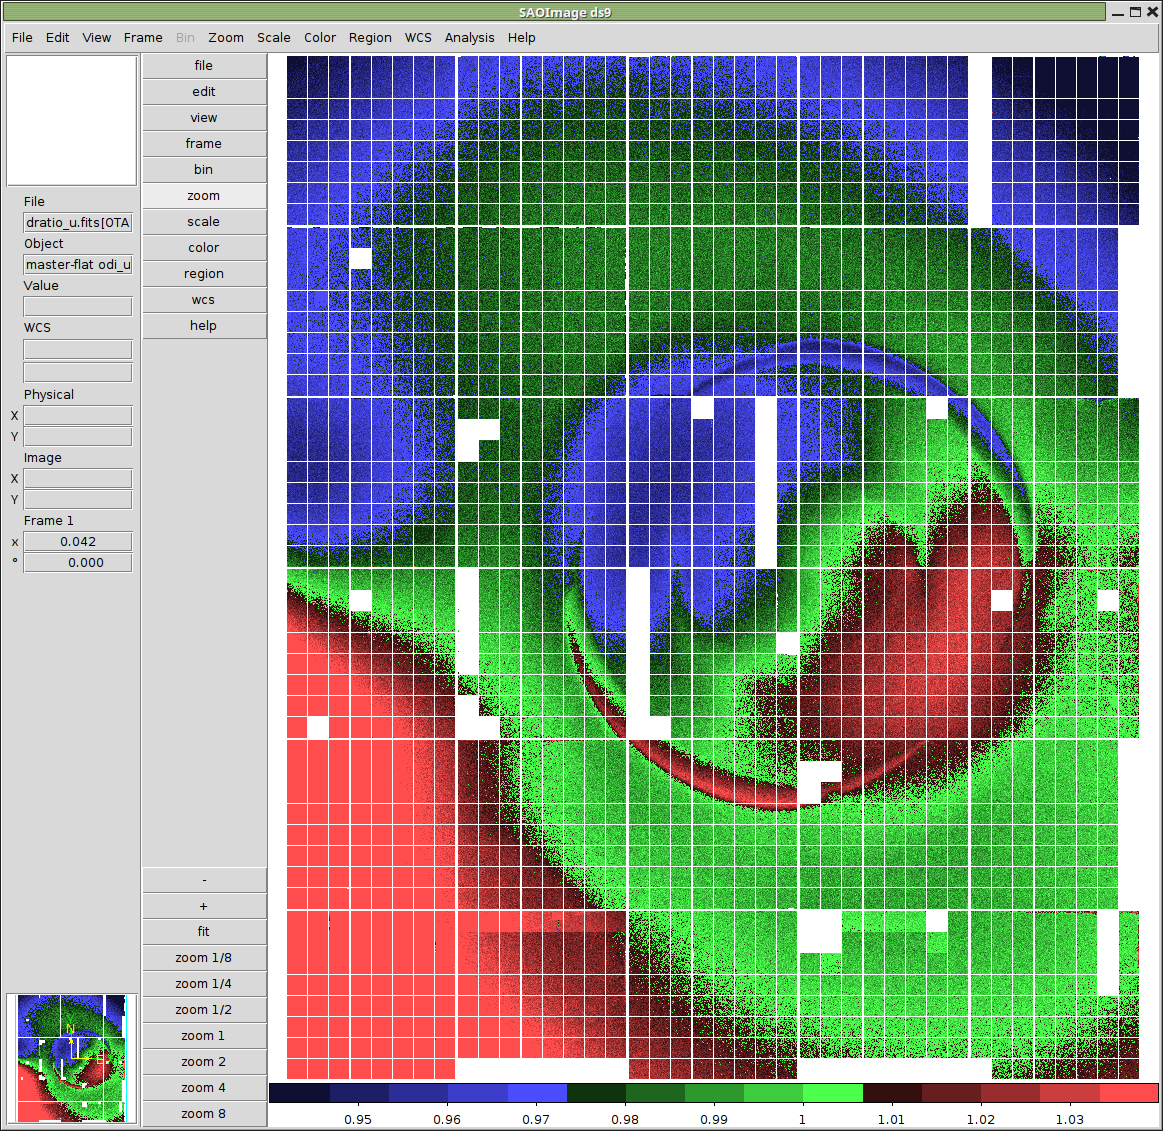
\includegraphics[width=0.2\textwidth]{images/nobaffle_u.png} &
                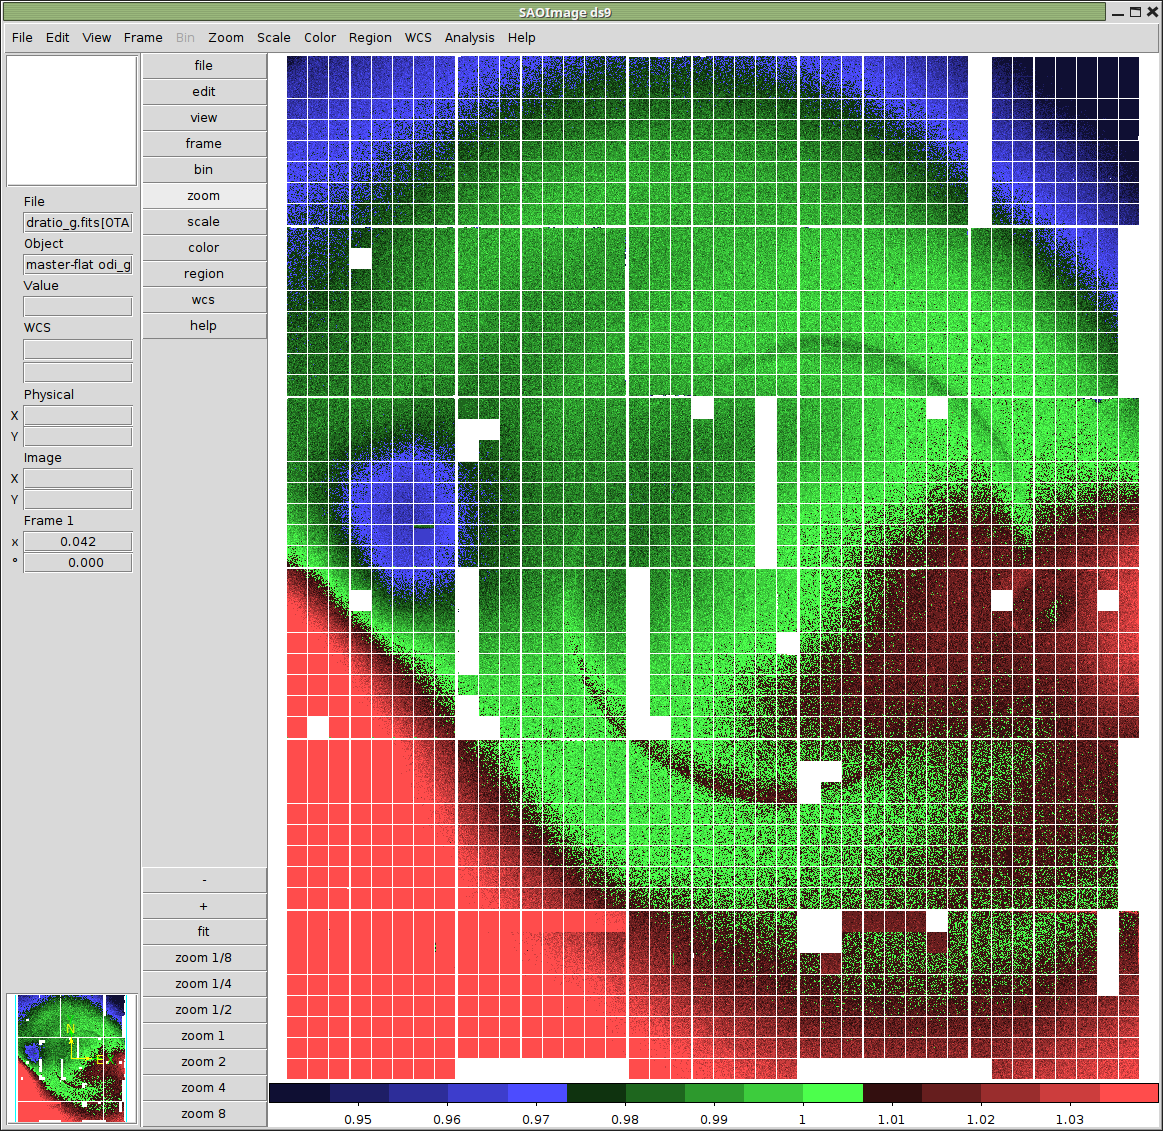
\includegraphics[width=0.2\textwidth]{images/nobaffle_g.png} &
                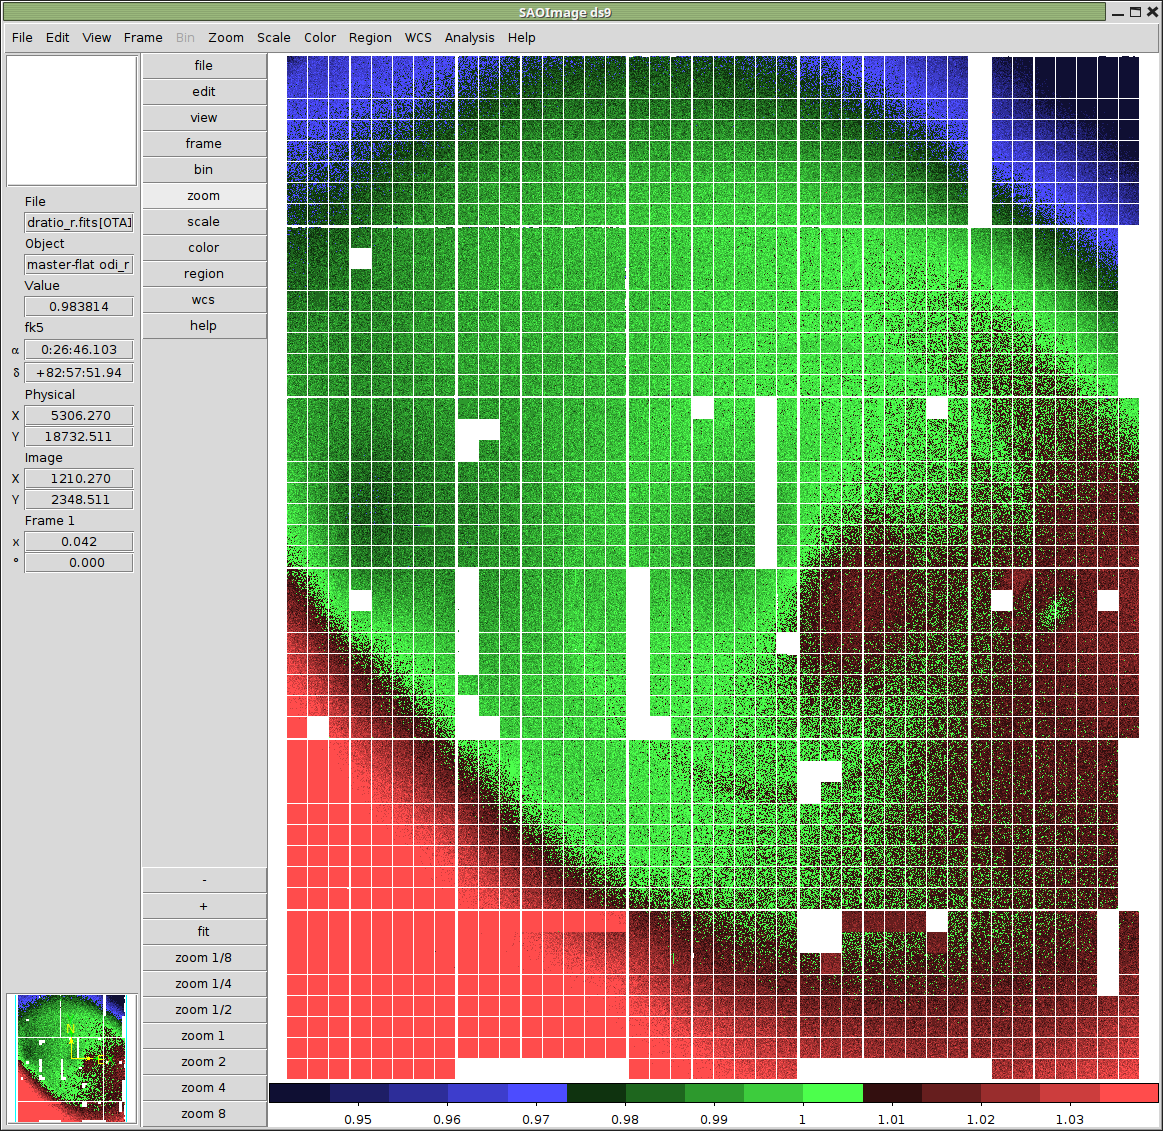
\includegraphics[width=0.2\textwidth]{images/nobaffle_r.png} &
                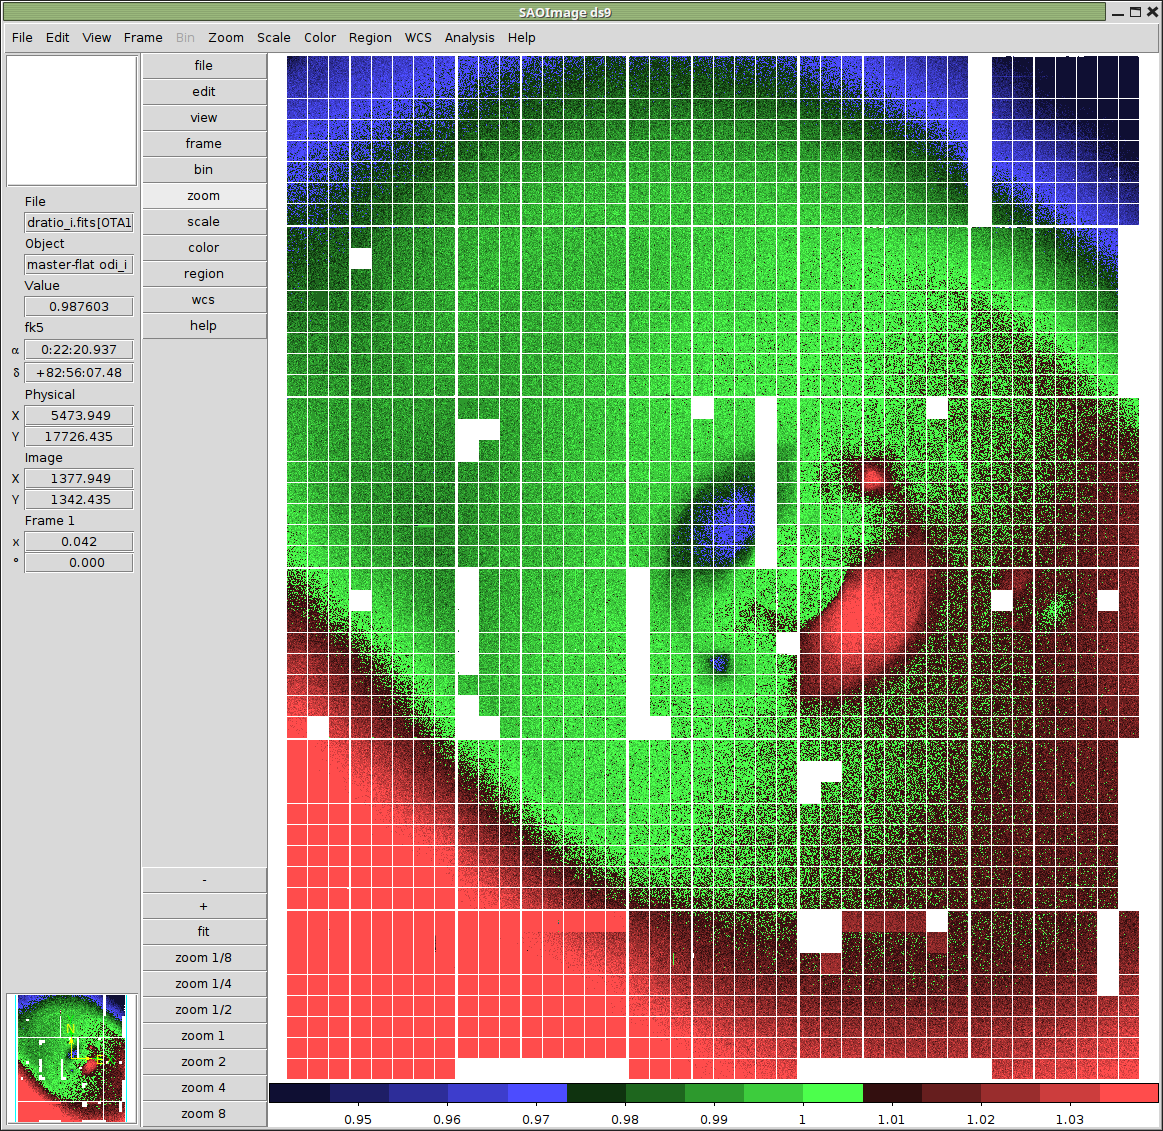
\includegraphics[width=0.2\textwidth]{images/nobaffle_i.png} &
                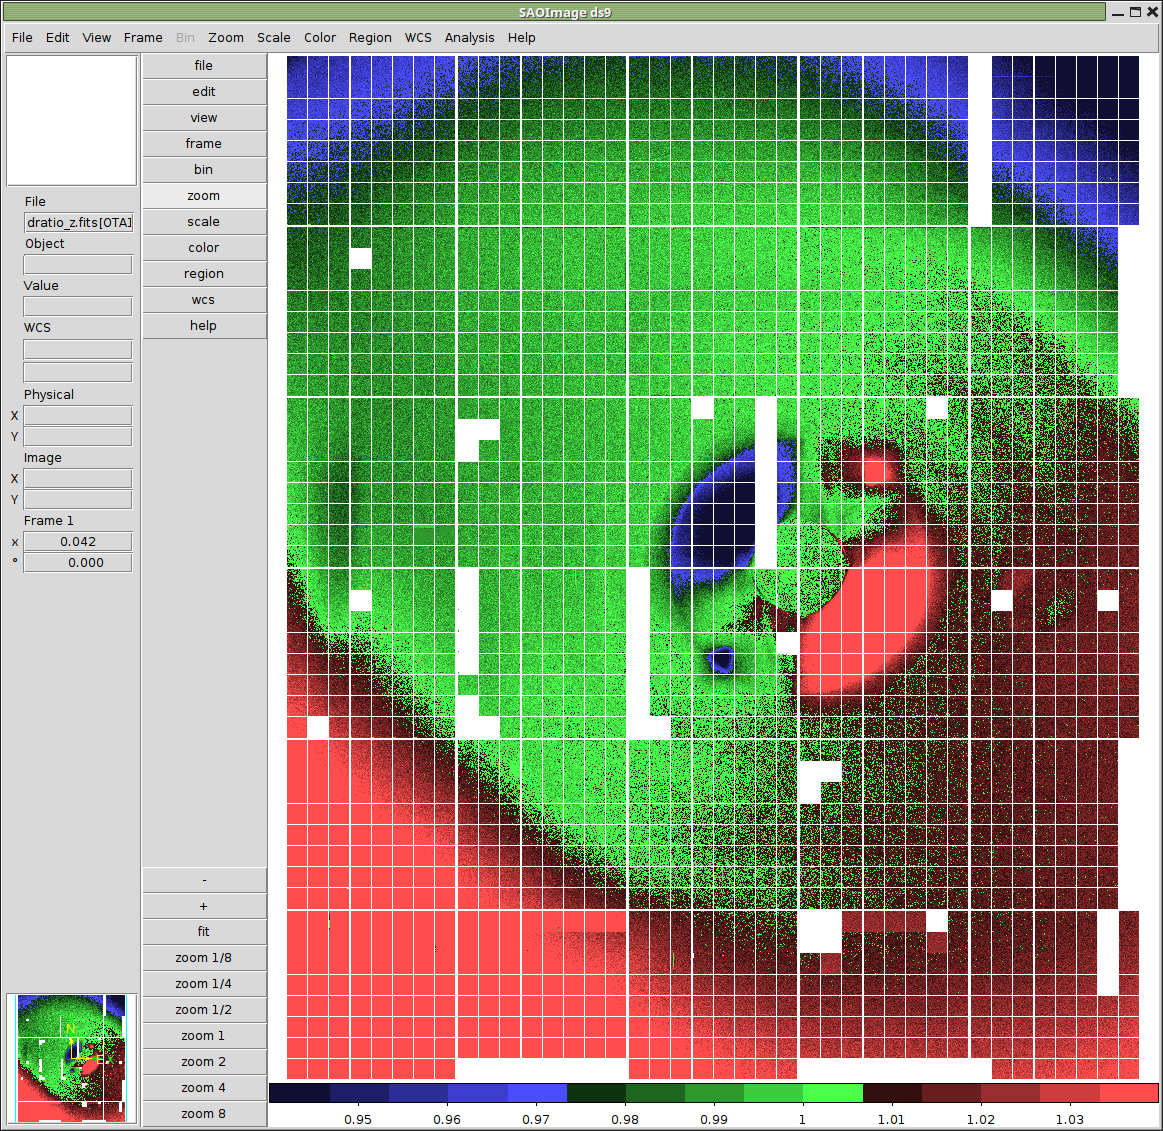
\includegraphics[width=0.2\textwidth]{images/nobaffle_z.png} \\
                \hline
                
            \end{tabular}
            
            \caption{\label{fig_flatfieldbaffle} Ratios of flat field images
                taken at an instrument rotator angle of $+90^\circ$ $-90^\circ$ 
                for all ODI broad band filters. }
            
        \end{figure}
        
    \end{landscape} \clearpage% Flush page
}




\subsection{Pupil ghost suppression using a two-bladed shutter}

\begin{figure}[h]
    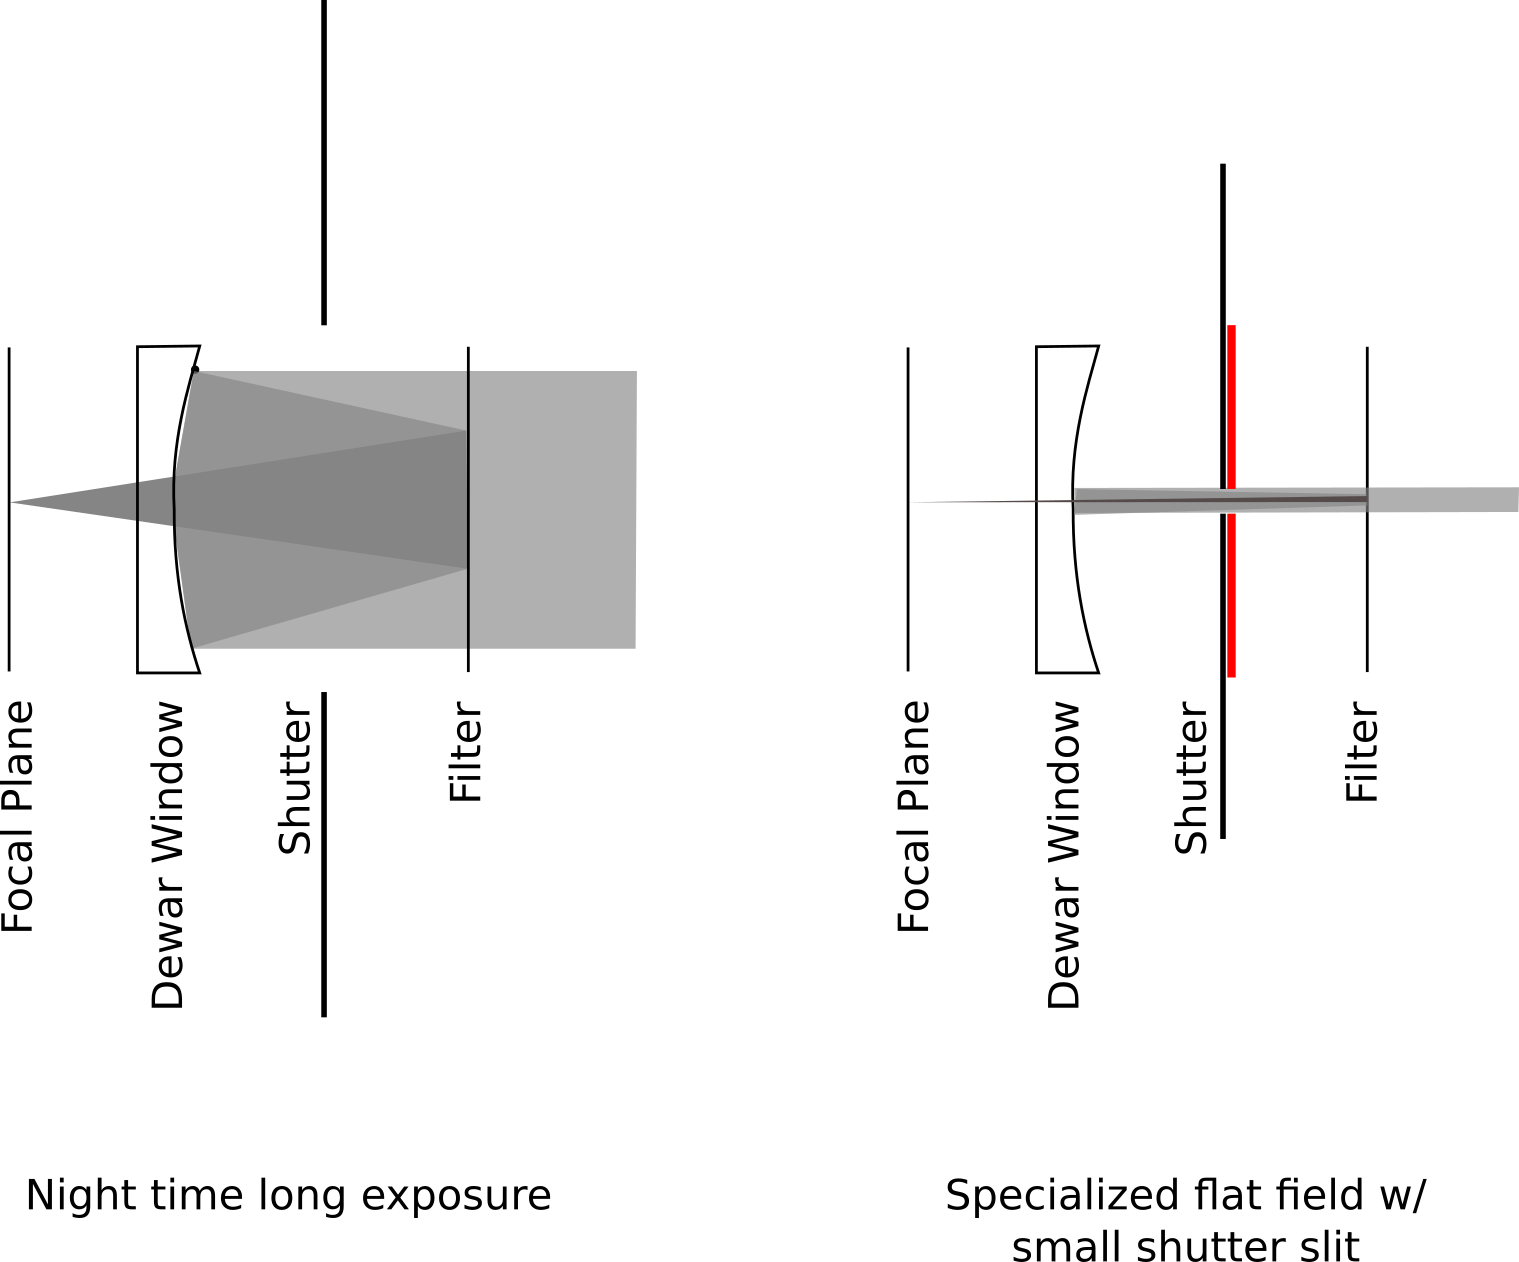
\includegraphics[height=8cm]{images/odishutterpupilghostsupression.png}
    \hspace{0.5cm} 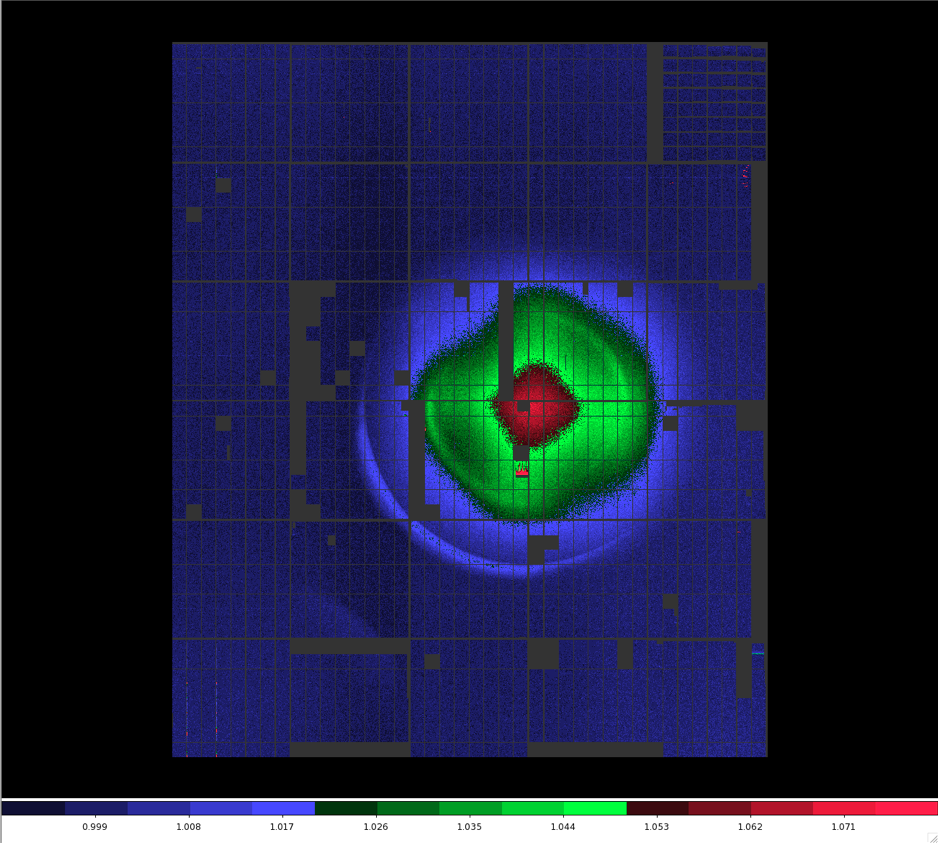
\includegraphics[height=8cm]{images/odi_layeronepg.png}
    \caption{ Left: Formation of the pupil ghost in ODI: a light component
        entering the instrument from the telescope (from the right) reflects of the
        concave dewar window, and the converging beam reflects of the filter and
        will create an in-focus image of the telescope pupil. Right: Ratio of a flat
        field taken with different shutter modes. The sensitivity variations between
        pixels and detectors cancel out, but the excess ghosting light remains. Note
        that this ratio shows the ghosting component created by filters that are at
        a different location than in Fig. 1, and the pupil ghost is largely out of
        focus.} \end{figure}

Reflections of the optical surfaces within WIYN One Degree Imager (ODI)
produce internal ghosting, i.e., flat fields1 or exposures of the night sky
will produce an image of the telescope pupil. Thanks to anti-reflection
coatings on the optics, each reflection is suppressed to about about 1\%-2\%
level, depending on the actual wavelength of the light, but the residual
light is still capable of producing a significant ghosting component. ODI’s
dewar window is concave, and paired with the plane surface of the passband
filter forms an imaging system that produces a focussed image of the
telescope pupil on the focal plane (see Fig. 1, left, for the ghost image
formation; see Fig. 2 for an example of an actual raw flat field image of
ODI affected by a pupil ghost image).

The excess light of the pupil ghost is undesirable for several reasons: In
night-sky observations it will produce an extra background component, but it
can be subtracted out. More severely, the pupil ghost also produces an extra
light component in a calibrating flat field, and if not treated, would lead
to a wrong sensitivity calibration in the affected areas.

The first method of choice to remove the pupil ghost out of calibration
images was to model the ghost image and to then subtract it out of the flat
field images. This approach was overall successful, but is is prone to
adding noise and residual errors from fitting a template to data.

The pupil ghost was found to be greatly suppressed by the ODI shutter2 when
the exposure is tuned in a way where the shutter blades mostly obstruct the
optical path in front of the dewar window, and expose only via a narrow slit
that moves slowly over the focal plane. There is a good video by the Bonn
shutter guys that demonstrates the exposure through a slit. This suppression
mechanism is illustrated by Fig. 1 (right). Note that, despite the shutter
forming only a narrow slit, the direct illumination of the focal plane is
identical to a flat field where the shutter completely opens.

This ghost-suppressing behavior of the shutter has been exploited already by
using very short exposure times of order of 50ms for sky flat fields, and
this new method has replaced the pupil ghost model subtraction method over
the last half year. However, this method was applicable only for situations
with a very bright flat field illumination that would support extremely
short exposure times. By lowering the travel speed of the shutter blades,
however, one can achieve the same ghost suppressing property at longer
exposure times on the focal plate. The cost, however, is that each flat
field will take about 27 seconds longer, as this is the travel time of the
blades (the travel time at default speed is about 0.75 seconds).

A good demonstration of the pupil ghost suppression by the shutter is to
divide a flat field where the shutter is operated conventionally by a flat
field where the shutter was operated in the narrow-slit mode. Other than in
the raw image of a flat field as in Fig. 1, the sensitivity variations
between pixels and detectors should dive out. Only the extra stray light
component should remain visible in the image. And voilà, Fig. 3 shows a
well-defined ghosting component, demonstrating that we can now generate
calibration flat fields that are free of internal reflections.


\subsection{Condensation}

remains issue, operational limit lowered to 70\% until full mitigation
strategy implemented.



\section{Infrastructure upgrades}

Lessons from pODI operations and early 5x6 ODI implemented:

- Helium compressors on UPS: cascade of failures: power outage leads to cooling outage leads to 
cold trap outgassing leads to vacuum interlock failure leads to warm up leads to the dark side. 

- Redundant dry air compressor and buffer tank for condensation prevention. Again. power outages 
and failures in compressor (mostly relay) had let to interruption in dry air supply.  Electronic 
data logging and alerting on dry air humidity.




\section{Summary}


%%%% References %%%%%
\bibliography{odi} 
\bibliographystyle{spiejour}

\end{document}
